%
%Не забыть:
%--------------------------------------
%Вставить колонтитулы, поменять название на титульнике



%--------------------------------------

\documentclass[a4paper, 12pt]{article} 

%--------------------------------------
%Russian-specific packages
%--------------------------------------
%\usepackage[warn]{mathtext}
\usepackage[T2A]{fontenc}
\usepackage[utf8]{inputenc}
\usepackage[english]{babel}
\usepackage[intlimits]{amsmath}
\usepackage{esint}
%--------------------------------------
%Hyphenation rules
%--------------------------------------
\usepackage{hyphenat}
\hyphenation{ма-те-ма-ти-ка вос-ста-нав-ли-вать}
%--------------------------------------
%Packages
%--------------------------------------
\usepackage{amsmath}
\usepackage{amssymb}
\usepackage{amsfonts}
\usepackage{amsthm}
\usepackage{latexsym}
\usepackage{mathtools}
\usepackage{etoolbox}%Булевые операторы
\usepackage{extsizes}%Выставление произвольного шрифта в \documentclass
\usepackage{geometry}%Разметка листа
\usepackage{indentfirst}
\usepackage{wrapfig}%Создание обтекаемых текстом объектов
\usepackage{fancyhdr}%Создание колонтитулов
\usepackage{setspace}%Настройка интерлиньяжа
\usepackage{lastpage}%Вывод номера последней страницы в документе, \lastpage
\usepackage{soul}%Изменение параметров начертания
\usepackage{hyperref}%Две строчки с настройкой гиперссылок внутри получаеммого
\usepackage[usenames,dvipsnames,svgnames,table,rgb]{xcolor}% pdf-документа
\usepackage{multicol}%Позволяет писать текст в несколько колонок
\usepackage{cite}%Работа с библиографией
\usepackage{subfigure}% Человеческая вставка нескольких картинок
\usepackage{tikz}%Рисование рисунков
\usetikzlibrary{circuits} % подключаем библиотеки, содержащие
\usetikzlibrary{circuits.ee} % УГО для схем
\usetikzlibrary{circuits.ee.IEC}
\usetikzlibrary{arrows} % подключаем библиотеки со стрелками
\usetikzlibrary{patterns} % и со штриховкой
\usepackage{float}% Возможность ставить H в положениях картинки
% Для картинок Моти
\usepackage{misccorr}
\usepackage{lscape}
\usepackage{cmap}
\usepackage{bm}
\newtheorem{definition}{Definition}



\usepackage{graphicx,xcolor}
\graphicspath{{Pictures/}}
\DeclareGraphicsExtensions{.pdf,.png,.jpg}

%----------------------------------------
%Список окружений
%----------------------------------------
\newenvironment {theor}[2]
{\smallskip \par \textbf{#1.} \textit{#2}  \par $\blacktriangleleft$}
{\flushright{$\blacktriangleright$} \medskip \par} %лемма/теорема с доказательством
\newenvironment {proofn}
{\par $\blacktriangleleft$}
{$\blacktriangleright$ \par} %доказательство
%----------------------------------------
%Список команд
%----------------------------------------
\newcommand{\grad}
{\mathop{\mathrm{grad}}\nolimits\,} %градиент

\newcommand{\diver}
{\mathop{\mathrm{div}}\nolimits\,} %дивергенция

\newcommand{\rot}
{\ensuremath{\mathrm{rot}}\,}

\newcommand{\Def}[1]
{\underline{\textbf{#1}}} %определение

\newcommand{\RN}[1]
{\MakeUppercase{\romannumeral #1}} %римские цифры

\newcommand {\theornp}[2]
{\textbf{#1.} \textit{ #2} \par} %Написание леммы/теоремы без доказательства

\newcommand{\qrq}
{\ensuremath{\quad \Rightarrow \quad}} %Человеческий знак следствия

\newcommand{\const}{\text{const}} % Написание const в формулах

\newcommand{\qlrq}
{\ensuremath{\quad \Leftrightarrow \quad}} %Человеческий знак равносильности

\renewcommand{\phi}{\varphi} %Нормальный знак фи

\renewcommand{\epsilon}{\varepsilon}

\newcommand{\me}
{\ensuremath{\mathbb{E}}}

\newcommand{\md}
{\ensuremath{\mathbb{D}}}



%\renewcommand{\vec}{\overline}




%----------------------------------------
%Разметка листа
%----------------------------------------
\geometry{top = 3cm}
\geometry{bottom = 2cm}
\geometry{left = 1.5cm}
\geometry{right = 1.5cm}
%----------------------------------------
%Колонтитулы
%----------------------------------------
\pagestyle{fancy}%Создание колонтитулов
\fancyhead{}
%\fancyfoot{}
\fancyhead[R]{\textsc{Сholesteriс Liquid Photonic Crystalls}}%Вставить колонтитул сюда
%----------------------------------------
%Интерлиньяж (расстояния между строчками)
%----------------------------------------
%\onehalfspacing -- интерлиньяж 1.5
%\doublespacing -- интерлиньяж 2
%----------------------------------------
%Настройка гиперссылок
%----------------------------------------
\hypersetup{				% Гиперссылки
unicode=true,           % русские буквы в раздела PDF
pdftitle={Заголовок},   % Заголовок
pdfauthor={Author},      % Автор
pdfsubject={Subject},      % Тема
pdfcreator={Creatir}, % Создатель
pdfproducer={Producer}, % Производитель
pdfkeywords={keyword1} {key2} {key3}, % Ключевые слова
colorlinks=false,       	% false: ссылки в рамках; true: цветные ссылки
linkcolor=blue,          % внутренние ссылки
citecolor=blue,        % на библиографию
filecolor=magenta,      % на файлы
urlcolor=blue           % на URL
}
%----------------------------------------
%Работа с библиографией 
%----------------------------------------
\renewcommand{\refname}{Список литературы}%Изменение названия списка литературы для article
%\renewcommand{\bibname}{Список литературы}%Изменение названия списка литературы для book и report
%----------------------------------------
\begin{document}
\begin{titlepage}
\begin{center}
$$$$
$$$$
$$$$
$$$$
{\Large{NATIONAL RESEARCH UNIVERSITY}}\\
\vspace{0.1cm}
{\Large{HIGHER SCHOOL OF ECONOMICS}}\\
\vspace{0.25cm}
{\large{Faculty of Physics}}\\
\vspace{5.5cm}
{\Huge\textbf{{Report}}}\\%Общее название
\vspace{1cm}
{\LARGE{<<Сholesteriс Liquid Photonic Crystalls>>}}\\%Точное название
\vspace{1cm}
{\large{M. I. Blumenau}}\\%Me
\vspace{2cm}
\vfill

\includegraphics[width = 0.2\textwidth]{HSElogo}\\
\vfill
Moscow\\
2021
\end{center}
\end{titlepage}

\tableofcontents
\newpage
\addcontentsline{toc}{section}{Introduction}
\section*{Introduction}
A liquid crystal (LC) is a specific aggregate state of a substance in which it exhibits both the properties of a crystal (anisotropy) and a liquid (fluidity). There are two types of liquid crystals:  lyotropic and thermotropic. Thermotropic LC is divided into three large classes: nematic, cholesteric, and smectic. 

In this report, the subject of the study was cholesteric photonic liquid crystals. They are formed by optically active molecules. The direction of the long axes of the molecules in each subsequent layer is a certain angle with the direction of the axes of the molecules of the previous layer. In this case, a spiral is formed, the step of which depends on the nature of the molecules and external influences. The step of the spiral corresponds to the rotation of the orientation axis of the molecules by $360^{\circ}$. A photonic crystal is a structure characterized by a periodic change in the value of the dielectric constant. Such structures are characterized by the presence of allowed and forbidden zones for the photon energy, due to the difference in the permittivity in the medium or the structure. This work aimed to obtain an experimental transmission spectrum of a liquid crystal (cholesteric).
\begin{figure}[H]
\centering
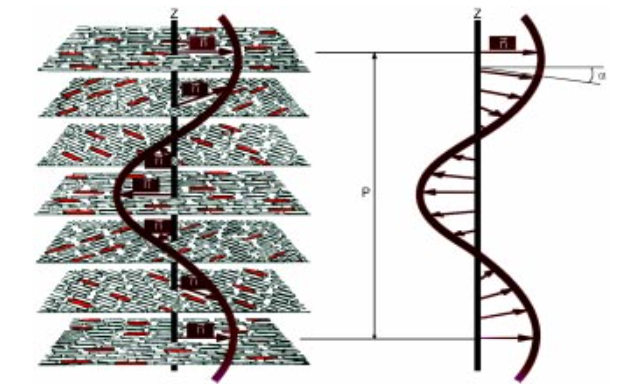
\includegraphics[width=1\linewidth]{Spiral.png}
\caption{Packaging of rod-shaped molecules
in cholesterol \cite{jk}}
\label{fig:1}
\end{figure}
\addcontentsline{toc}{section}{Theoretical information}
\section*{Theoretical information}
The most natural way to describe the optical properties of CLC is to solve the Maxwell equations (with the boundary conditions corresponding to the problem. The dielectric properties of CLC are described by the coordinate-dependent permittivity tensor  $\hat{\mathbf{\epsilon}} (\mathbf{r})$. The dependence of the tensor on the coordinates consists in the change from point to point in the orientation of the main axes of the tensor, the local direction of which is determined by the orientation of the CLC molecules at the point under consideration.
For a perfect cholesteric structure, $\hat{\mathbf{\epsilon}} (\mathbf{r})$ has the form:
\begin{equation}\label{epsten}
\begin{pmatrix}
\overline{\epsilon} +  \overline{\epsilon} \delta cos(\tau z)& \pm \overline{\epsilon} \delta sin(\tau z) & 0\\
\pm \overline{\epsilon} \delta sin(\tau z) & \overline{\epsilon} -  \overline{\epsilon} \delta cos(\tau z) & 0\\
0 & 0 & \epsilon_{3}
\end{pmatrix}
\end{equation}
where the $z$ axis is directed along the optical axis, $\tau = 4 \pi / p$, where p is the step of the cholesteric helix, $\epsilon_{3} = \epsilon_{2}, \epsilon_{1}$ are the main values of the permittivity tensor, $\overline{\epsilon} = (\epsilon_{1} + \epsilon_{2})/2$ and $\delta =  (\epsilon_{1} - \epsilon_{2})/(\epsilon_{1} + \epsilon_{2})$. As can be seen from (\ref{epsten}), the period of change in the dielectric properties of the CLC is equal to half a step. The two signs correspond to two geometric possibilities: the plus of the right and the minus of the left cholesteric helix.

They obtain solutions of the Maxwell equations in the CLC with dielectric permittivity (\ref{epsten}). For a wave propagating along the optical axis, the equations take the form 
\begin{equation}
\frac{\partial^{2} \overrightarrow{E}}{\partial z^{2}}=\frac{\hat{\mathbf{\epsilon}}}{c^{2}} \frac{\partial^{2} \overrightarrow{E}}{\partial t^{2}},	
\end{equation}
where the $z$ axis is directed along the optical axis, $\overrightarrow{E}$ the vector of the electric field in the medium, perpendicular in this case to the $z$ axis. 

Next, they search for the field in the crystal in the form of a superposition of two plane waves:
\begin{equation}
\overrightarrow{E}=\mathbf{n}_{+} E_{+} \exp \left[i\left(\beta+\frac{\tau}{2}\right) z-i \omega t\right]+\mathbf{n}_{-} E_{-} \exp \left[i\left(\beta-\frac{\tau}{2}\right) z-i \omega t\right]
\end{equation}
where $\mathbf{n}_{\pm}=\left(\sigma \pm i \pi_{0}\right) / \sqrt{2}$ are the orts of circular polarizations, $\omega$ - the frequency of light, i.e. the solution is sought in the form of a Bloch wave, as required by the periodicity of the CLC. For the amplitudes, the following system of equations is obtained:
\begin{equation}\label{sys}
\begin{array}{l}
{\left[\kappa^{2}-\left(\beta+\frac{\tau}{2}\right)^{2}\right] E_{+}+\kappa^{2} \delta E_{-}=0} \\
\kappa^{2} \delta E_{+}+\left[\kappa^{2}-\left(\beta-\frac{\tau}{2}\right)^{2}\right] E_{-}=0
\end{array}
\end{equation}
where $\kappa^{2} = \omega^{2} \overline{\epsilon} / c^{2}$. A system has non-zero solutions when its determinant is zero.
From (\ref{sys}), they obtain an expression that defines as a function of the wave frequency, the spiral period, and the anisotropy parameter:
\begin{equation}\label{sol}
\beta_{j}=\pm \sqrt{x^{2}+\frac{\tau^{2}}{4} \pm x \sqrt{\tau^{2}+x^{2} \delta^{2}}}, \quad j=1,2,3,4
\end{equation}

In the case of normal incidence, the boundary conditions are that the electric field and the magnetic field are continuous at the crystal boundaries. Let a wave $\overrightarrow{E} i=\left(E_{+}^{i} \mathbf{n}_{+}+E_{-}^{i} \mathbf{n}_{-}\right) e^{i\left(\kappa_{0} z-\omega t\right)}$ fall on the crystal, where $\kappa_{0}$ is the wave vector in the medium surrounding the crystal, and $E_{+}^{i}$, $E_{-}^{i}$ are the amplitudes of the right- and left-polarized components in the incident wave. The general solution of the equation for the field in a crystal has the form 
\begin{equation}
\overrightarrow{E}(z, t)=e^{-i \omega t} \sum_{j=1}^{4}\left(E_{+}\right)_{j}\left(\mathbf{n}_{+} e^{i\left[\beta_{j}+(\tau / 2)\right] z}+\xi_{j} \mathbf{n}_{-} e^{i\left[\beta_{j}-(\tau / 2)\right]z}\right),
\end{equation}
where $\xi_{j} = (E_{-}/E_{+})_{j} = \kappa^{2} \delta / ((\beta_{j} - \tau/2)^{2} - \kappa^{2})$.

The amplitudes of the reflected and transmitted waves are searched for in the form
\begin{equation}
\overrightarrow{E}^{r}=\left(E_{+}^{r} \mathbf{n}_{-}+E_{-}^{r} \mathbf{n}_{+}\right) e^{-i\left(\kappa_{0} z+\omega t\right)}, \quad \overrightarrow{E}^{t}=\left(E_{+}^{t} \mathbf{n}_{+}+E_{-}^{t} \mathbf{n}_{-}\right) e^{i\left(\kappa_{0} z-\omega t\right)}
\end{equation}
Solving the boundary problem in this way (counting the right-hand cholesterol spiral for certainty), we will see that the left-polarized wave "excites" only solution 1 or 4  (\ref{sol}) in the crystal (depending on which side it falls on the crystal) and penetrates the CLC without experiencing selective reflection. The right-polarized wave excites two eigenwaves 2 and 3 (\ref{sol}) in the crystal.
The transmission coefficient $T$ (for a non-absorbing crystal) is determined by the expression
\begin{equation}
T=\left|\frac{E_{+}^{t}}{E_{+}^{i}}\right|^{2}=\frac{\tau^{2} \beta^{2}}{\tau^{2} \beta^{2}+\kappa^{4} \delta^{2} \sin ^{2} \beta L}
\end{equation}
where L is thickness of the LC, $\beta^{2}=\kappa^{2}+\left(\tau^{2} / 4\right)-\kappa \sqrt{\tau^{2}+\kappa^{2} \delta^{2}}$. For frequencies in the forbidden zones $\beta^{2} < 0$, so $sin(\beta L)$ turns to $i sinh(|\beta| L)$. \cite{bel}
\addcontentsline{toc}{section}{Equipment and methods}
\section*{Equipment and methods}
I used a spectrometer from the Avantes AvaSpec StarLine family, a converging lens, an incandescent lamp, and an aperture. The light from the lamp was limited by the aperture, then it was focused with the help of a converging lens. Liquid crystal was held in a specific casing and mounted on a holder to be exactly in the focus point of the lens. The results were collected by AvaSoft8 and later processed with Python. Schematic diagram of the installation attached below:
\begin{figure}[H]
\centering
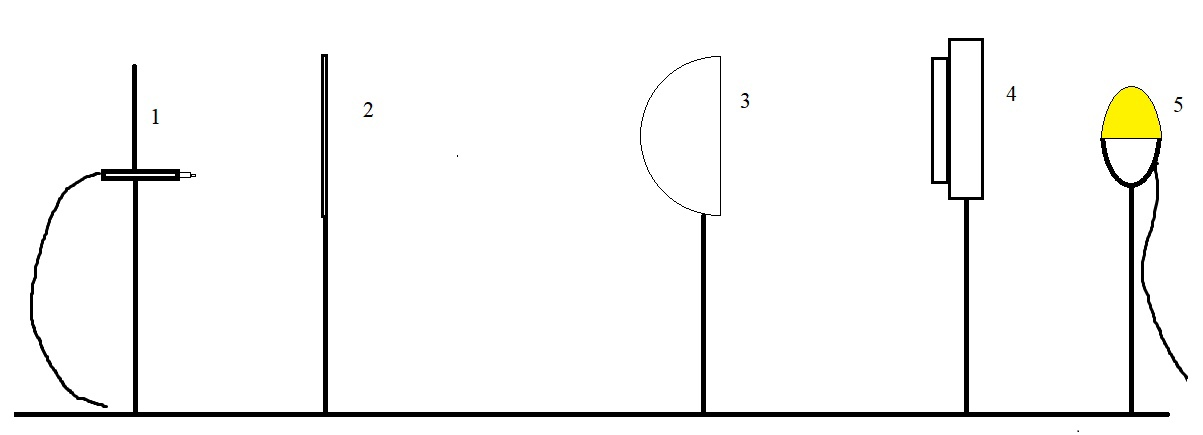
\includegraphics[width=1\linewidth]{Principle.jpg}
\caption{The layout of the optical elements in the experiment. The figure shows the following elements: 1~ -- waveguide; 2~ -- LC; 3~-- collecting lens; 4~ -- diaphragm; 5~ -- incandescent lamp}
\label{fig:2}
\end{figure}
Source code link: \href{https://github.com/burunduk387/HSE-FF/tree/main/LabOptics/CLC}{https://github.com/burunduk387/HSE-FF/tree/main/LabOptics/CLC}
\addcontentsline{toc}{section}{Experimental results}
\section*{Experimental results}
I had two CLCs. They were different in size, so I will refer to them as "Small" and "Large", respectively. 

As for the small CLC, the results are: $\delta = 0.095$, $n = 1.62$, $L = 5.51$ mkm. The graph below shows the theoretical curve and actual experiment data plotted on a colored background.
\begin{figure}[H]
\centering
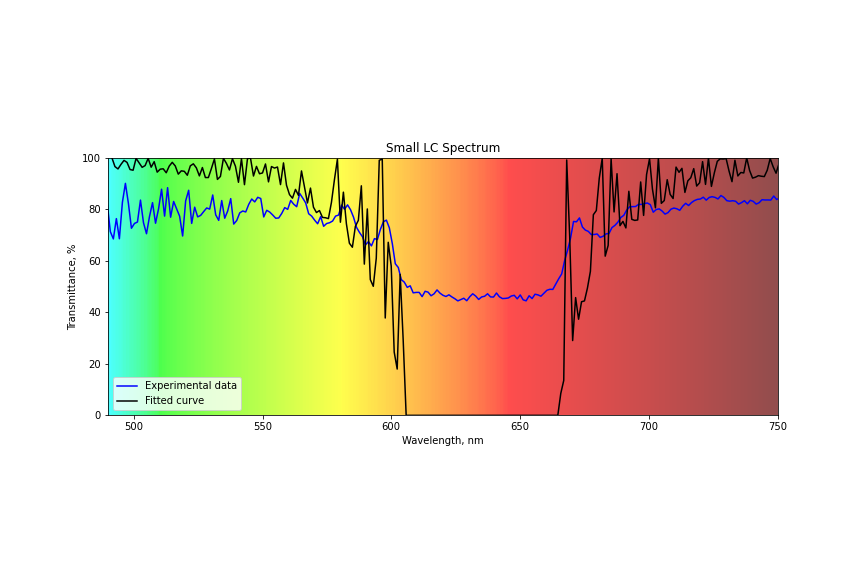
\includegraphics[width=1\linewidth]{SmallLC.png}
\caption{Small LC transmittance}
\label{fig:3}
\end{figure}
For the large CLC: $\delta = 0.11$, $n = 1.65$, $L = 20$ mkm.

\begin{figure}[H]
\centering
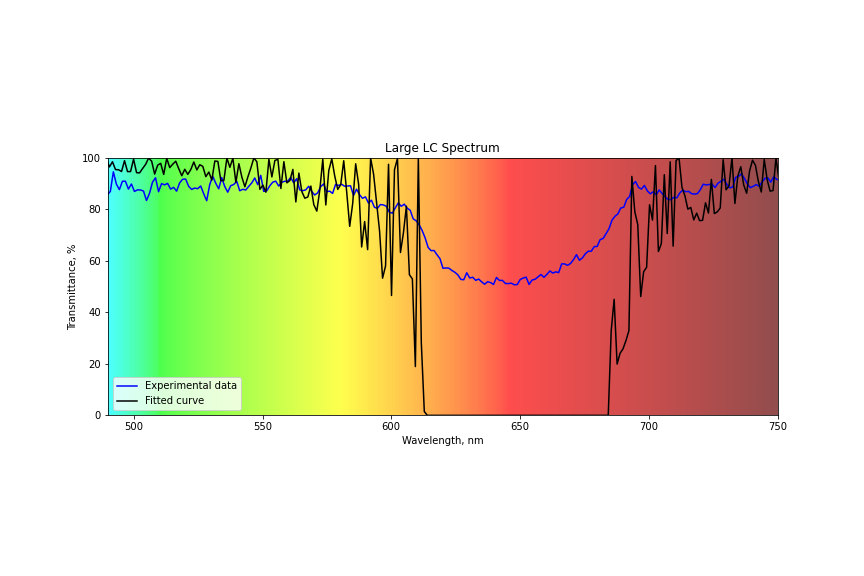
\includegraphics[width=1\linewidth]{LargeLC.png}
\caption{Large LC transmittance}
\label{fig:4}
\end{figure}
It can be seen that the theoretical spectrum constructed according to formulas qualitatively describes the features of a cholesteric liquid crystal, but does not give accurate results. In my opinion, it can be explained: the theory does not take into account the absorption available in the substance used, the reflection of the glass, and the fact that in this experiment no polarizers were used. Moreover, due to some numerical problems (to be more specific, the default float-precision on modern systems), the value of the function cannot be estimated precisely, which leads to even more dissimilarities.

\addcontentsline{toc}{section}{Conclusion}
\section*{Conclusion}
I attempted to calculate the transmittance of two CLCs. Although crystals are different at a first glance, they showed similar results. I got: 
\begin{center} 

\begin{tabular}{|c|c|c|c|} 
\hline 
Size & $\delta$ & $n$ & $L$, mkm \\ 
\hline 
S & 0.095 & 1.62 & 5.51 \\ 
\hline 
L & 0.11 & 1.65 & 20\\
\hline 
\end{tabular} 

\end{center}
It was possible to find the difference in crystal thickness. Other parameters are similar in order of magnitude. Unfortunately, due to the disadvantages of the applied theory and technical problems, it is difficult to say whether the results are correct or not.
\addcontentsline{toc}{section}{References}
\begin{thebibliography}{9}
\bibitem{bel} 
V. A. Belyakov, V, E. Dmitrienko, V. P. Orlov. 
Optics of Cholesteric Liquid Crystals.
Advances in the physical sciences, 1979.
\bibitem{jk} 
V. P. Shibaev. 
Liquid Crystals: Cholesteric. 
Chemistry and life, 2008.
\end{thebibliography}
\end{document}
